\PassOptionsToPackage{hyphens}{url}
\documentclass[compress,aspectratio=169]{beamer}

%\usetheme{Goettingen} % Generates a sidebar that is replaced by a header bar in the given theme
\usepackage[official]{eurosym}
\usepackage{multirow}
\usepackage{units}
\usepackage{../assets/beamerthemeGoettingen} % make sure the theme file is on this path
\usepackage{tikz}
\usetikzlibrary{shapes}
\usepackage{menukeys}
\definecolor{bgcolor}{HTML}{E0E0E0}
\newcommand{\console}[1]{
  \colorbox{bgcolor}{\texttt{#1}}
}
\graphicspath{{../}{../assets/}}


% --- document configuration ---
\newcommand{\mytitle}{Introduction to Git}     
% Leave empty for no subtitle
\newcommand{\mysubtitle}{A free and open source VCS}
\newcommand{\myauthor}{Jonathan Decker}
\newcommand{\myauthorurl}{jonathan.decker@uni-goettingen.de}
\newcommand{\myvenue}{PCHPC}
% For example, use \today
\newcommand{\mydate}{2023.04.17}
% For example, Institute for Computer Science / GWDG
\newcommand{\myinstitute}{Institute for Computer Science / GWDG}
% Leave empty for no footer image
\newcommand{\myfooterimage}{}
\newcommand{\mygrouplogo}{hps-logo}
% Images must be enabled manually under title page \titleLogo
% Adjust position and width manually for fewer images
\newcommand{\mytitleimageone}{}
\newcommand{\mytitleimagetwo}{}
\newcommand{\mytitleimagethree}{}


% --- title page ---
\title{\Large \mytitle}
\venue{\myvenue}
\date{\mydate}
\subtitle{\mysubtitle}
\authorURL{\myauthorurl}
\author{{\myauthor}}
\authorFooter{\myauthor \hspace{0.3cm} \includegraphics[height=1em]{\myfooterimage}}
\institute{\myinstitute}
\groupLogo{\includegraphics[width=2cm]{\mygrouplogo}}
\titleLogo{
%\includegraphics[height=2.7cm]{\mytitleimageone}
%\includegraphics[height=2.7cm]{\mytitleimagetwo}
%\includegraphics[height=2.7cm]{\mytitleimagethree}
}

\setbeamertemplate{footline}[text line]{
\begin{beamercolorbox}[sep=0.5em,wd=\paperwidth,leftskip=0.2cm,rightskip=0.1cm]{footlinecolor}
\myauthor \hfill \insertVenue \hfill \insertframenumber\,/\,\inserttotalframenumber%\ref{pg:lastpage}
\end{beamercolorbox}
}

\begin{document}

\begin{frame}[plain]
	\titlepage
\end{frame}

\begin{frame}[t]{Table of contents}
  \tableofcontents[subsectionstyle=hide/hide]
\end{frame}

% --- slides begin ---

\begin{frame}{Learning Objectives}
  \begin{itemize}
    \item Know the purpose of VCS in general and Git in particular
    \item Set up and configure Git
    \item Create local and clone remote repositories
    \item Craft and review commits
    \item Interact with local and remote branches
  \end{itemize}
\end{frame}

\section{Introduction}

\begin{frame}
  \frametitle{Why version control systems (VCS)?}
  \begin{itemize}
    \item Track changes in your project
    \item Be able to jump to the last known working state
    \item Explore different (potentially experimental ``throwaway'') branches of development
    \item Attach meaningful notes to each set of changes aka. ``commit''
    \item Collaborate with others
  \end{itemize}
\end{frame}
\begin{frame}{What is Git?}
  \begin{minipage}[t]{0.3\linewidth}
      \only<1>{\raisebox{-\height}{\includegraphics[width=4cm]{assets/Git-logo-2007-eps-converted-to.pdf}}}
      \only<2->{\raisebox{-\height}{\includegraphics[width=4cm]{assets/Git-Logo-2Color-eps-converted-to.pdf}}}
      \visible<4>{\raisebox{-10em}{\hspace{1cm}\includegraphics[width=2cm]{assets/progit2.png}}}
  \end{minipage}\hfill
  \begin{minipage}[t]{0.7\linewidth}
      \begin{itemize}
          \item Initial release in 2005 by Linus Torvalds
          \item Used for developing the Linux Kernel 
          \item Previously: \textsc{BitKeeper} (proprietary)
          \item<3-> \url{https://git-scm.com/}
              \begin{itemize}
                  \item Documentation
                  \item \textsc{Git} command reference
                  \item<4> Ebook: \textit{Scott Chacon, Ben Straub - Pro Git}
              \end{itemize}
      \end{itemize}
  \end{minipage}
  % \only<1>{\raisebox{-.5cm}{\tiny Von Git - http://git-scm.com/downloads/logos, GPL (\href{https://de.wikipedia.org/wiki/Git\#/media/File:Git-logo-2007.svg})}}
  % \only<2->{\raisebox{-.5cm}{\tiny Git Logo by \href{http://twitter.com/jasonlong}{\textcolor{gwdg}{Jason Long}} is licensed unter the \href{http://creativecommons.org/licenses/by/3.0/}{\textcolor{gwdg}{Creative Commons Attribution 3.0 Unported License}}.}}
\end{frame}
\begin{frame}
  \frametitle{Git terminology}
  \begin{itemize}
    \item Git projects are called \textit{repositories}.
    \item Fully distributed, i.e. each local clone contains the entire project history
    \item Versions of the managed file tree are called \textit{commit}s.
    \item They form a graph where each new commit has at least one parent.
    \item Branches are easily created - they're just named pointers to commits.
    \item \texttt{HEAD} points to the branch that will receive the next commit.
    \item Important commits (e.g. release versions) can get a named (even annotated, signed) \textit{tag} pointing to them.
  \end{itemize}
\end{frame}

\begin{frame}
  \frametitle{Fundamental Structure: Directed Acyclic Graph (DAG) of commits}
  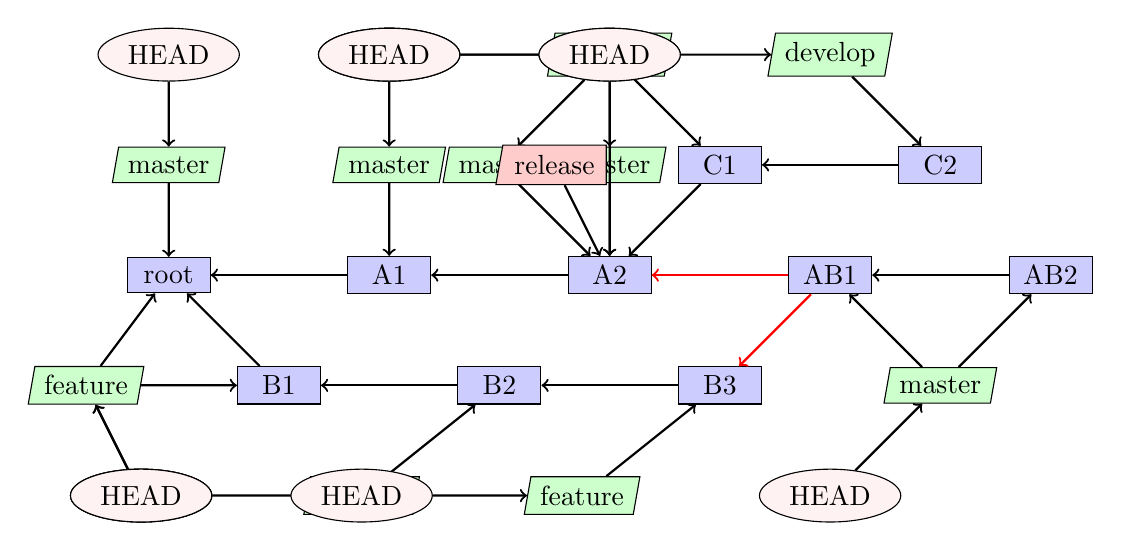
\begin{tikzpicture}[scale=.7]
      \tikzstyle{commit} = [draw, rectangle, fill=blue!20, minimum width=3em];
      \tikzstyle{branch} = [draw, trapezium, trapezium left angle=80, trapezium right angle=100, fill=green!20, minimum width=4em];
      \tikzstyle{tag} = [draw, trapezium, trapezium left angle=80, trapezium right angle=90, fill=red!20, minimum width=4em];
      \tikzstyle{head} = [draw, ellipse, fill=pink!20];
      \tikzstyle{link} = [->, thick];

      % commits: master
      \node at (0,0) [commit] (commit-master-1) {root};

      \visible<2->{%
          \node at (4,0) [commit] (commit-master-2) {A1};
          \draw[link] (commit-master-2) -- (commit-master-1);
      }
      \visible<3->{%
          \node at (8,0) [commit] (commit-master-3) {A2};
          \draw[link] (commit-master-3) -- (commit-master-2);
      }

      %commits: feature
      \visible<5->{%
          \node at (2, -2) [commit] (commit-feature-1) {B1};
          \draw[link] (commit-feature-1) -- (commit-master-1);
      }
      \visible<6->{%
          \node at (6, -2) [commit] (commit-feature-2) {B2};
          \draw[link] (commit-feature-2) -- (commit-feature-1);
      }
      \visible<7->{%
          \node at (10, -2) [commit] (commit-feature-3) {B3};
          \draw[link] (commit-feature-3) -- (commit-feature-2);
      }

      % commits: master
      \visible<12->{%
          \node at (12,0) [commit] (commit-master-4) {AB1};
          \draw[link,color=red] (commit-master-4) -- (commit-master-3);
          \draw[link,color=red] (commit-master-4) -- (commit-feature-3);
      }
      \visible<13->{%
          \node at (16,0) [commit] (commit-master-5) {AB2};
          \draw[link] (commit-master-5) -- (commit-master-4);
      }

      % commits: develop
      \visible<9->{%
          \node at (10,2) [commit] (commit-develop-1) {C1};
          \draw[link] (commit-develop-1) -- (commit-master-3);
      }
      \visible<10->{%
          \node at (14,2) [commit] (commit-develop-2) {C2};
          \draw[link] (commit-develop-2) -- (commit-develop-1);
      }

      % branch: master
      \visible<1>{%
          \node at (0,2) [branch] (branch-master-1) {master};
          \draw[link] (branch-master-1) -- (commit-master-1);
      }
      \visible<2>{%
          \node at (4,2) [branch] (branch-master-2) {master};
          \draw[link] (branch-master-2) -- (commit-master-2);
      }
      \visible<3-7>{%
          \node at (8,2) [branch] (branch-master-3) {master};
          \draw[link] (branch-master-3) -- (commit-master-3);
      }
      \visible<8-11>{%
          \node at (6,2) [branch] (branch-master-4) {master};
          \draw[link] (branch-master-4) -- (commit-master-3);
      }
      \visible<12->{%
          \node at (14,-2) [branch] (branch-master-5) {master};
      }
      \visible<12>{%
          \draw[link] (branch-master-5) -- (commit-master-4);
      }
      \visible<13->{%
          \draw[link] (branch-master-5) -- (commit-master-5);
      }

      % branch: feature
      \visible<4-5>{%
          \node at (-1.5,-2) [branch] (branch-feature-1) {feature};
      }
      \visible<4>{%
          \draw[link] (branch-feature-1) -- (commit-master-1);
      }
      \visible<5>{%
          \draw[link] (branch-feature-1) -- (commit-feature-1);
      }
      \visible<6>{%
          \node at (3.5,-4) [branch] (branch-feature-2) {feature};
          \draw[link] (branch-feature-2) -- (commit-feature-2);
      }
      \visible<7->{%
          \node at (7.5,-4) [branch] (branch-feature-3) {feature};
          \draw[link] (branch-feature-3) -- (commit-feature-3);
      }

      % branch: develop
      \visible<8-9>{%
          \node at (8,4) [branch] (branch-develop-1) {develop};
      }
      \visible<8>{%
          \draw[link] (branch-develop-1) -- (commit-master-3);
      }
      \visible<9>{%
          \draw[link] (branch-develop-1) -- (commit-develop-1);
      }
      \visible<10->{%
          \node at (12,4) [branch] (branch-develop-2) {develop};
          \draw[link] (branch-develop-2) -- (commit-develop-2);
      }

      % head
      \visible<1>{%
          \node at (0,4) [head] (head) {HEAD};
          \draw[link] (head) -- (branch-master-1);
      }
      \visible<2>{%
          \node at (4,4) [head] (head) {HEAD};
          \draw[link] (head) -- (branch-master-2);
      }
      \visible<3>{%
          \node at (8,4) [head] (head) {HEAD};
          \draw[link] (head) -- (branch-master-3);
      }
      \visible<4>{%
          \node at (-0.5,-4) [head] (head) {HEAD};
          \draw[link] (head) -- (branch-feature-1);
      }
      \visible<5>{%
          \node at (-0.5,-4) [head] (head) {HEAD};
          \draw[link] (head) -- (branch-feature-1);
      }
      \visible<6>{%
          \node at (-0.5,-4) [head] (head) {HEAD};
          \draw[link] (head) -- (branch-feature-2);
      }
      \visible<7>{%
          \node at (3.5,-4) [head] (head) {HEAD};
          \draw[link] (head) -- (branch-feature-3);
      }
      \visible<8-9>{%
          \node at (4,4) [head] (head) {HEAD};
          \draw[link] (head) -- (branch-develop-1);
      }
      \visible<8-9>{%
          \node at (4,4) [head] (head) {HEAD};
          \draw[link] (head) -- (branch-develop-1);
      }
      \visible<10-11>{%
          \node at (8,4) [head] (head) {HEAD};
      }
      \visible<10>{%
          \draw[link] (head) -- (branch-develop-2);
      }
      \visible<11>{%
          \draw[link] (head) -- (branch-master-4);
      }
      \visible<12->{%
          \node at (12,-4) [head] (head) {HEAD};
          \draw[link] (head) -- (branch-master-5);
      }

      % tag: release
      \visible<14>{%
          \node at (7,2) [tag] (tag-1) {release};
          \draw[link] (tag-1) -- (commit-master-3);
      }
  \end{tikzpicture}
\end{frame}

% \begin{frame}{Git Structure: Repository Directory}
%   \begin{minipage}[t]{0.5\linewidth}
%       working copy (excerpt)\\
%       \begin{tikzpicture}[scale=.5]
%           \tikzstyle{label} = [anchor=west];
%           \tikzstyle{link} = [->];
%           \draw (0,0) -- (0,-13);

%           \draw (0,-1) -- (1,-1);
%           \node at (1,-1) [label] {\texttt{.git}};
%           \draw (0.5,-1) -- (0.5,-10);

%           \draw (0.5,-2) -- (1.5,-2);
%           \node at (1.5,-2) [label] {\texttt{config}};

%           \draw (0.5,-3) -- (1.5,-3);
%           \node at (1.5,-3) [label] {\texttt{HEAD}};

%           \draw (0.5,-4) -- (1.5,-4);
%           \node at (1.5,-4) [label] {\texttt{objects}};
%           \draw (1,-4) -- (1,-9);

%           \draw (1,-5) -- (2,-5);
%           \node at (2,-5) [label] {\texttt{00}};
%           \draw (1.5,-5) -- (1.5,-8);

%           \draw (1.5,-6) -- (2.5,-6);
%           \node at (2.5,-6) [label] {\texttt{0...0} (38 hex digits)};
%           \node at (2.5,-7.25) [label] {\texttt{~...}};
%           \draw (1.5,-8) -- (2.5,-8);
%           \node at (2.5,-8) [label] {\texttt{f...f}};

%           \draw (1,-9) -- (2,-9);
%           \node at (2,-9) [label] {\texttt{ff}};
%           \draw (1.5,-9) -- (1.5,-9.5);

%           \draw (0.5,-10) -- (1.5,-10);
%           \node at (1.5,-10) [label] {\texttt{refs}};
%           \draw (1,-10) -- (1,-12);

%           \draw (1,-11) -- (2,-11);
%           \node at (2,-11) [label] {\texttt{heads}};
%           \draw (1.5,-11) -- (1.5,-11.5);

%           \draw (1,-12) -- (2,-12);
%           \node at (2,-12) [label] {\texttt{tags}};
%           \draw (1.5,-12) -- (1.5,-12.5);

%           \draw (0,-13) -- (1,-13);
%           \node at (1,-13) [label] {(tree given by HEAD)};
%       \end{tikzpicture}
%   \end{minipage}\hfill
%   \begin{minipage}[t]{0.5\linewidth}
%       \begin{itemize}
%           \item Distributed VCS: Working copy contains entire history.
%           \item objects stored according to their SHA-1 checksum
%           \item HEAD/branches/tags: files with target's checksum.
%           \item bare repository: no working copy, just contents of .git
%       \end{itemize}
%   \end{minipage}
% \end{frame}

\section{Setup and Configuration}

\begin{frame}
  \frametitle{Installing Git}
  \begin{itemize}
    \item \textbf{Linux distributions}\\Use your package manager of choice, e.g. \texttt{apt install git}
    \item \textbf{MacOS}\\Installation is possible via Homebrew: \texttt{brew install git}
    \item \textbf{Windows}\\Download and run the Git installer \url{https://git-scm.com/download/win}
  \end{itemize}
\end{frame}

\begin{frame}
  \frametitle{Configuring Git}
  \begin{itemize}
    \item First, we make sure that git is installed and ready to use:\\
      \console{git -\phantom{}-version}
    \item Each commit contains your name \texttt{<NAME>} and mail adress \texttt{<EMAIL>}, so let's set those:\\
      \console{git config -\phantom{}-global user.name "<NAME>"}\\
      \console{git config -\phantom{}-global user.email "<EMAIL>"}\\
      Omitting the \texttt{-\phantom{}-global} switch would configure them for your current repo.
  \end{itemize}
\end{frame}

\section{Creating commits}

\begin{frame}
  \frametitle{Creating and cloning repositories}
  \begin{itemize}
    \item We can locally create a new, empty repository with\\\console{git init}\\The commit objects and other internal Git data will be stored in a hidden subdirectory \texttt{.git}.
    \item Usually we'd like to get a local copy of a remote repo at \texttt{<URL>}, done via\\\console{git clone <URL>}
    \item There are many options to show the history leading to the commit \texttt{<C>}, e.g.:\\\console{git log -\phantom{}-decorate -\phantom{}-graph -\phantom{}-oneline [<C>]}
      \begin{itemize}
        \item Without specifying any commits, the history to the current commit is shown.
        \item There are many GUIs available as well, cf. \url{https://git-scm.com/downloads/guis}
      \end{itemize}
  \end{itemize}
\end{frame}

\begin{frame}
  \frametitle{Creating commits}
  \begin{itemize}
    \item The current state of the working directory can be queried as follows:\\\console{git status}\\This will show changed and new, untracked files.
    \item Best practice for files that are produced by your build:
      \begin{itemize}
        \item Include in \texttt{.gitignore} file and don't commit them.
        \item These files can be bootstrapped for most programming languages at \url{gitignore.io}.
        \item Examples: \texttt{*.o} for a C project or \texttt{*.pdf} for \LaTeX
      \end{itemize}
    \item To \textit{stage} all changed files, i.e. mark as part of the next commit:\\\console{git add .}
      \begin{itemize}
        \item Replace \console{.} by a filename (pattern) to be more specific
      \end{itemize}
    \item Finally, we can create the new commit with:\\\console{git commit -m "<MESSAGE>"}
  \end{itemize}
\end{frame}

\section{Managing branches}

\begin{frame}
  \frametitle{Local and remote branches}
  \begin{itemize}
    \item Let's first get an overview of the available branches:\\\console{git branch}
    \item With the \console{-a} switch we get \textit{remote tracking} branches as well.
    \item A new branch \texttt{<BRANCH>} can be created with\\\console{git branch <BRANCH>}
    \item ...and selected as the current one (i.e. representing the working tree) with\\\console{git checkout <BRANCH>}
    \item In order to merge in the commits from \texttt{<OTHER\_BRANCH>} we use\\\console{git merge <OTHER\_BRANCH>}
      \begin{itemize}
        \item Git is really smart about automatically resolving merge conflicts, at least for text files.
        \item If this fails, we have to manually edit the colloding files and then create the merge commit.
      \end{itemize}
  \end{itemize}
\end{frame}

\begin{frame}
  \frametitle{Local and remote branches}
  \begin{itemize}
    \item Remote repositories can be shown with:\\\console{git remote}
      \begin{itemize}
        \item With the \console{-v} switch each URL is shown as well.
      \end{itemize}
    \item When cloning a git repo, the source is automatically configured as the remote \texttt{origin}.
    \item We can configure a new remote \texttt{<REMOTE>} at \texttt{<URL>} as follows:\\\console{git remote add <REMOTE> <URL>}
    \item The \texttt{<URL>} can be given by
      \begin{itemize}
        \item a web tool like \textit{GitHub}, \textit{GitLab} or \textit{Gitea} or
        \item the path to a \textit{bare} repo (created with \console{git init -\phantom{}-bare} and not containing a working tree).
      \end{itemize}
  \end{itemize}
\end{frame}

\begin{frame}
  \frametitle{Local and remote branches}
  \begin{itemize}
    \item Showing branches with full verbosity reveals \textit{remote tracking branches}:\\\console{git branch -vv}\\Again, these are automatically created when cloning from a remote repo.
    \item In order to update the remote tracking branch:\\\console{git fetch}
    \item This can be combined to automatically merge into the local branch:\\\console{git pull}
    \item Finally, we can upload locally new commits to the remote branch with:\\\console{git push}
    \item Tracking can be set manually, e.g. for \texttt{<BRANCH>} to track \texttt{<REMOTE>} with:\\\console{git push -u <REMOTE> <BRANCH>}
  \end{itemize}
\end{frame}

\end{document}
